%%%%%%%%%%%%%%%%%%%%%%%%%%%%%%%%%%%%%%%%%
% University Assignment Title Page 
% LaTeX Template
% Version 1.0 (27/12/12)
%
% This template has been downloaded from:
% http://www.LaTeXTemplates.com
%
% Original author:
% WikiBooks (http://en.wikibooks.org/wiki/LaTeX/Title_Creation)
%
% License:
% CC BY-NC-SA 3.0 (http://creativecommons.org/licenses/by-nc-sa/3.0/)
% 
% Instructions for using this template:
% This title page is capable of being compiled as is. This is not useful for 
% including it in another document. To do this, you have two options: 
%
% 1) Copy/paste everything between \begin{document} and \end{document} 
% starting at \begin{titlepage} and paste this into another LaTeX file where you 
% want your title page.
% OR
% 2) Remove everything outside the \begin{titlepage} and \end{titlepage} and 
% move this file to the same directory as the LaTeX file you wish to add it to. 
% Then add \input{./title_page_1.tex} to your LaTeX file where you want your
% title page.
%
%%%%%%%%%%%%%%%%%%%%%%%%%%%%%%%%%%%%%%%%%
%\title{Title page with logo}
%----------------------------------------------------------------------------------------
%   PACKAGES AND OTHER DOCUMENT CONFIGURATIONS
%----------------------------------------------------------------------------------------

\documentclass[12pt]{article}
\usepackage[english]{babel}
\usepackage[utf8x]{inputenc}
\usepackage{amsmath}
\usepackage{graphicx}
\usepackage[colorinlistoftodos]{todonotes}
\usepackage{placeins}


\begin{document}

\begin{titlepage}

\newcommand{\HRule}{\rule{\linewidth}{0.5mm}} % Defines a new command for the horizontal lines, change thickness here

\center % Center everything on the page
 
%----------------------------------------------------------------------------------------
%   HEADING SECTIONS
%----------------------------------------------------------------------------------------

\textsc{\LARGE Aalto University}\\[1.5cm] % Name of your university/college
\textsc{\Large T-75.4400 Information retrieval}\\[0.5cm] % Major heading such as course name
\textsc{\large Assignment 2}\\[0.5cm] % Minor heading such as course title

%----------------------------------------------------------------------------------------
%   TITLE SECTION
%----------------------------------------------------------------------------------------

\HRule \\[0.4cm]
{ \huge \bfseries Comparing ranking methods for information retrieval}\\[0.4cm] % Title of your document
\HRule \\[1.5cm]
 
%----------------------------------------------------------------------------------------
%   AUTHOR SECTION
%----------------------------------------------------------------------------------------

\begin{minipage}{0.45\textwidth}
\begin{center} \large
Antti \textsc{Partanen}\\ % Your name
\texttt{antti.partanen@aalto.fi}\\
295967
\end{center}
\end{minipage}
~
\begin{minipage}{0.45\textwidth}
\begin{center} \large
Vikram \textsc{Kamath}\\ % Supervisor's Name
\texttt{vikram.kamath@aalto.fi}\\
XXXXXX
\end{center}
\end{minipage}\\[2cm]


% If you don't want a supervisor, uncomment the two lines below and remove the section above
%\Large \emph{Author:}\\
%John \textsc{Smith}\\[3cm] % Your name

%----------------------------------------------------------------------------------------
%   DATE SECTION
%----------------------------------------------------------------------------------------

{\large \today}\\[2cm] % Date, change the \today to a set date if you want to be precise

%----------------------------------------------------------------------------------------
%   LOGO SECTION
%----------------------------------------------------------------------------------------


\includegraphics{AaltoSCI_EN_9.pdf}\\[1cm] % Include a department/university logo - this will require the graphicx package
 
%----------------------------------------------------------------------------------------

\vfill % Fill the rest of the page with whitespace



\end{titlepage}

\todo[inline, color=green!40]{Too messy titlepage?}

\begin{abstract}
In this paper, we compare compare two ranking methods: VSM (Vector Space Model) and BM25 for document collection from ACM digital library database. Furthermore, we study the effects of morphological techniques, including stemmers and stop words.
\todo[inline, color=green!40]{Abstract maybe not necessary? Overlap with introduction?}
\end{abstract}

\section{Introduction}

The task of Information retrieval is to obtain information resources relevant to the imminent need from information resources. Resources include books, journals and other documents. Searches can be based on meta-data or on full-text indexing.

Automated information retrieval systems are used to reduce the so called \textit{information overload}, i.e. the difficulty of a person to understand an issue due to overwhelming amounts of information. Most existing text retrieval techniques rely on indexing key-words. Unfortunately keywords or index terms alone cannot adequately capture the document contents, resulting in poor retrieval performance. Yet, keyword indexing is widely used in commercial systems because it is still the most viable way by far to process large amount of text. 

Efficient and effective information retrieval techniques are critical in managing the increased amount of textual information available in electronic form. Therefore, it is no wonder that currently the most visible IR systems are web search engines.  

In this paper, we compare the two information retrieval techniques: Vector Space Model (VSM) and BM25. Furthermore, we analyze what effects does the usage of stemmers (porter stemmer) and stopwords have with the retrieval result. The evaluation of our experiments is visualized with eleven point precision recall curves. 

\todo[inline, color=green!40]{Draft version: aka needs modifying + references}

\section{Techniques}

Techniques that we used were VSM and BM25. 
\todo[inline, color=green!40]{Add text and references} 

\subsection{VSM}
\subsection{BM25}
\subsection{Stemmers}
\subsection{Stopwords}


\section{Evaluation}

\todo[inline, color=green!40]{Add text and charts}

\textbf{Precision}

\textbf{Recall}

\textbf{Eleven point precision recall curve}


\section{Conclusions}

\todo[inline, color=green!40]{Add conclusions}

\section{Contributions}

\todo[inline, color=green!40]{Mind map style of work division might look neat?}

\begin{figure}[p]
    \centering
    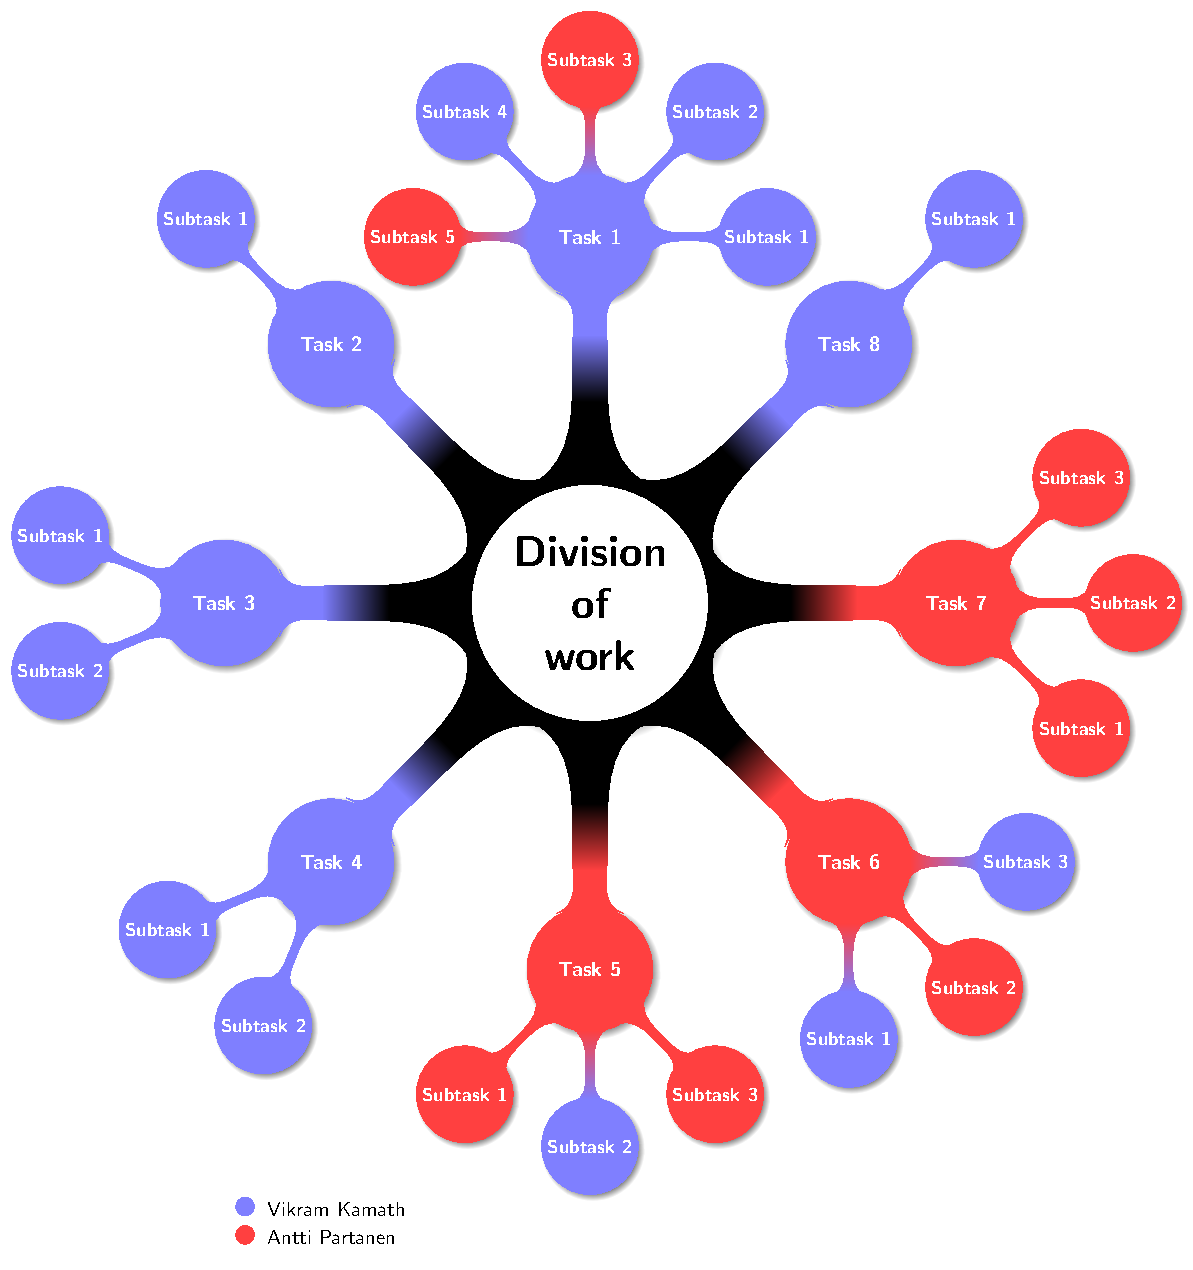
\includegraphics[scale=0.6]{contributions_tree.pdf}
    \caption{Contributions represented in a mindmap}
    \label{fig:contributions_tree}
\end{figure}
\FloatBarrier

%\begin{figure}[h]


\nocite{*}
\bibliographystyle{plain}
\bibliography{bibliography.bib}

\todo[inline, color=green!40]{Add more references}

\appendix
\section{Installation instructions} \label{App:instructions}

\todo[inline, color=green!40]{Add instructions}

Here is a brief systems installation and system configuration instructions. 

\begin{enumerate}

\item ...
\item ...

\end{enumerate}

\end{document}